\documentclass[10pt]{article}

\usepackage[T1]{fontenc}
\usepackage[left=2cm, right=2cm, top=2cm, bottom=2cm]{geometry}
\usepackage[skins]{tcolorbox}
\usepackage{hyperref, fancyhdr, lastpage, tocloft, ragged2e, multicol}
\usepackage{amsmath, amssymb, amsthm}
\usepackage{tkz-tab}

\def\pagetitle{Fonctions usuelles}

\title{\bf{\pagetitle}\\\large{Corrigé}}
\date{Septembre 2023}
\author{DARVOUX Théo}

\DeclareMathOperator{\ch}{ch}
\DeclareMathOperator{\sh}{sh}
\DeclareMathOperator{\tah}{th}
\DeclareMathOperator{\argth}{argth}

\hypersetup{
    colorlinks=true,
    citecolor=black,
    linktoc=all,
    linkcolor=blue
}

\pagestyle{fancy}
\cfoot{\thepage\ sur \pageref*{LastPage}}


\begin{document}
\renewcommand*\contentsname{Exercices.}
\renewcommand*{\cftsecleader}{\cftdotfill{\cftdotsep}}
\maketitle
\hrule
\tableofcontents
\vspace{0.5cm}
\hrule

\thispagestyle{fancy}
\fancyhead[L]{MP2I Paul Valéry}
\fancyhead[C]{\pagetitle}
\fancyhead[R]{2023-2024}
\allowdisplaybreaks

\pagebreak

\section*{Exercice 4.1 [$\blacklozenge\lozenge\lozenge$]}
\begin{tcolorbox}[enhanced, width=7in, center, size=fbox, fontupper=\large, drop shadow southwest]
    Soit $f:\mathbb{R}\rightarrow\mathbb{R}$ une fonction $2$-périodique et $3$-périodique. Montrer que $f$ est $1$-périodique.\\
    On a :
    \begin{align*}
        \forall{x\in\mathbb{R}}\begin{cases}x-2\in\mathbb{R}\\f(x-2)=f(x)\end{cases} \text{ et } \begin{cases}x+3\in\mathbb{R}\\f(x+3)=f(x)\end{cases}
    \end{align*}
    Alors :
    \begin{align*}
        \forall{x\in\mathbb{R}}\begin{cases}x-2+3\in\mathbb{R}\\f(x-2+3)=f(x-2)=f(x)\end{cases}
    \end{align*}
    \qed
\end{tcolorbox}

\addcontentsline{toc}{section}{Vocabulaire sur les fonctions.}
\addcontentsline{toc}{section}{\protect\numberline{}Exercice 4.1}

\section*{Exercice 4.2 [$\blacklozenge\blacklozenge\blacklozenge$]}
\begin{tcolorbox}[enhanced, width=7in, center, size=fbox, fontupper=\large, drop shadow southwest]
    Déterminer toutes les fonctions croissantes $f:\mathbb{R}\rightarrow\mathbb{R}$ telles que
    \begin{equation*}
        \forall{x\in\mathbb{R}} \hspace{0.25cm} f(f(x))=x.
    \end{equation*}
    Soit $x\in\mathbb{R}$ et $f$ une solution du problème.\\
    On remarque que $f:x\mapsto x$ est solution du problème.\\
    Supposons $f(x)>x$, on a : $f(f(x))>f(x)$ par croissance de $f$. Or $f(f(x))=x$ donc $x>f(x)$, ce qui est absurde.\\
    Supposons $f(x)<x$, on a : $f(f(x))<f(x)$ par croissance de $f$. Or $f(f(x))=x$ donc $x<f(x)$, ce qui est absurde.\\
    Ainsi, la seule fonction de $\mathbb{R}$ vers $\mathbb{R}$ solution est $f:x\mapsto x$.
\end{tcolorbox}
\addcontentsline{toc}{section}{\protect\numberline{}Exercice 4.2}

\section*{Exercice 4.3 [$\blacklozenge\lozenge\lozenge$] S'entraîner tout seul à dériver.}
\begin{tcolorbox}[enhanced, width=7in, center, size=fbox, fontupper=\large, drop shadow southwest]
    Pour chacune des fonctions ci-dessous, donner un ou plusieurs intervalles sur lesquels la fonction est dérivable, et préciser sa dérivée.
    \begin{center}
        $A:x\mapsto x^\pi,\hspace{0.5cm}B:x\mapsto\pi^x,\hspace{0.5cm}C:x\mapsto\cos(5x),\hspace{0.5cm}D:x\mapsto\tah(\ch(x))$,\\
        $E:x\mapsto\ln\left(1+x^3\right)n\hspace{0.5cm}F:x\mapsto\cos\left(\sqrt{\ln(x)}\right),\hspace{0.5cm}G:x\mapsto\frac{1}{\sqrt{3x-1}},\hspace{0.5cm}H:x\mapsto\sin|x+1|$.
    \end{center}
    
    $G':x\mapsto-\frac{3}{2}(3x-1)^{3/2}$
    
    \begin{itemize}
        \item $A':\begin{cases}\mathbb{R}^*_+\rightarrow\mathbb{R}\\x\mapsto\pi x^{\pi-1}\end{cases}$\hspace{1.8cm}• $D':\begin{cases}\mathbb{R}\rightarrow\mathbb{R}\\x\mapsto\frac{\sh(x)}{\ch^2(\ch(x))}\end{cases}$\hspace{1.6cm}• $H'_-:\begin{cases}]-\infty,-1[\rightarrow\mathbb{R}\\x\mapsto-\cos(-x-1)\end{cases}$
        \item $B':\begin{cases}\mathbb{R}\rightarrow\mathbb{R}\\x\mapsto\ln(\pi)\pi^x\end{cases}$\hspace{1.5cm}• $E':\begin{cases}\mathbb{R}\setminus\{1\}\rightarrow\mathbb{R}\\x\mapsto\frac{3x^2}{1+x^3}\end{cases}$\hspace{1.6cm}• $H'_+:\begin{cases}]1,+\infty[\rightarrow\mathbb{R}\\x\mapsto\cos(x+1)\end{cases}$
        \item $C':\begin{cases}\mathbb{R}\rightarrow\mathbb{R}\\x\mapsto-5\sin(5x)\end{cases}$\hspace{1.0cm}• $F':\begin{cases}]1,+\infty[\rightarrow\mathbb{R}\\x\mapsto\frac{\sin(\sqrt{\ln(x)})}{2x\sqrt{\ln(x)}}\end{cases}$
    \end{itemize}
\end{tcolorbox}

\addcontentsline{toc}{section}{Étude de fonctions.}
\addcontentsline{toc}{section}{\protect\numberline{}Exercice 4.3}
\section*{Exercice 4.4 [$\blacklozenge\lozenge\lozenge$]}
\begin{tcolorbox}[enhanced, width=7in, center, size=fbox, fontupper=\large, drop shadow southwest]
    Donner le tableau de variations complet de
    \begin{equation*}
        f:x\mapsto x^{x\ln(x)}.
    \end{equation*}
    On a :
    \begin{equation*}
        f:x\mapsto e^{x\ln^2(x)}
    \end{equation*}
    Donc :
    \begin{equation*}
        f':\begin{cases}\mathbb{R}_+^*\rightarrow\mathbb{R}\\x\mapsto\ln(x)(\ln(x)+2)e^{x\ln^2(x)}\end{cases}
    \end{equation*}
    Son tableau de variations est donc :
    \begin{center}
        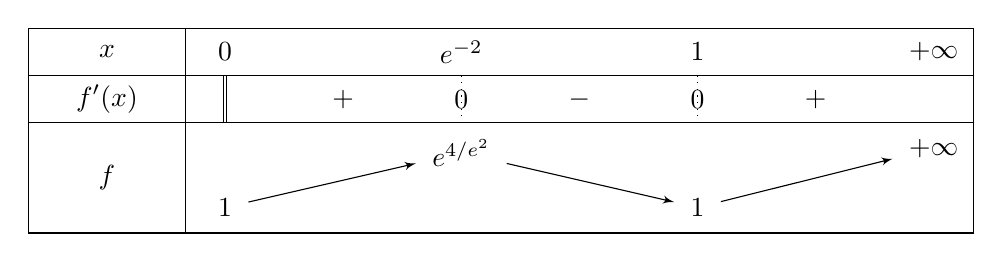
\begin{tikzpicture}
            \tkzTabInit[espcl=3]{$x$/0.6,$f'(x)$/0.6,$f$/1.4}{$0$,$e^{-2}$,$1$,$+\infty$}
            \tkzTabLine{d,+,z,-,z,+}
            \tkzTabVar{-/$1$,+/$e^{4/e^{2}}$,-/$1$,+/$+\infty$}
        \end{tikzpicture}
    \end{center}
\end{tcolorbox}
\addcontentsline{toc}{section}{\protect\numberline{}Exercice 4.4}

\section*{Exercice 4.5 [$\blacklozenge\blacklozenge\lozenge$]}
\begin{tcolorbox}[enhanced, width=7in, center, size=fbox, fontupper=\large, drop shadow southwest]
    1. Démontrer que
    \begin{equation*}
        \forall x\in]-1,+\infty[, \hspace{0.5cm} \frac{x}{1+x}\leq\ln(1+x)\leq x.
    \end{equation*}
    2. À l'aide du théorème des gendarmes, calculer $\lim\limits_{x\rightarrow0}{\frac{\ln(1+x)}{x}}$.\\
    3. Retrouver ce résultat en faisant apparaître un taux d'accroissement.\\[0.25cm]
    1. Posons :
    \begin{equation*}
        f:x\mapsto\frac{x}{1+x}-\ln(1+x) \hspace{2cm} g:x\mapsto\ln(1+x)-x
    \end{equation*}
    Elles sont dérivables et tout et tout :
    \begin{equation*}
        f':x\mapsto-\frac{x}{(1+x)^2} \hspace{2cm} g':x\mapsto-\frac{x}{1+x}
    \end{equation*}
    \begin{center}
        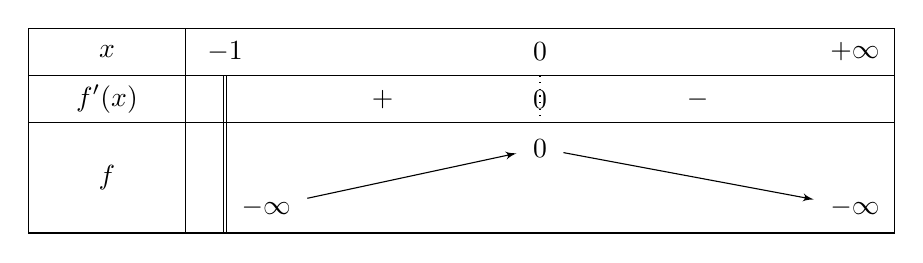
\begin{tikzpicture}
            \tkzTabInit[espcl=4]{$x$/0.6,$f'(x)$/0.6,$f$/1.4}{$-1$,0,$+\infty$}
            \tkzTabLine{d,+,z,-}
            \tkzTabVar{D-/$-\infty$, +/$0$, -/$-\infty$}
        \end{tikzpicture}
        \\[0.25cm]
        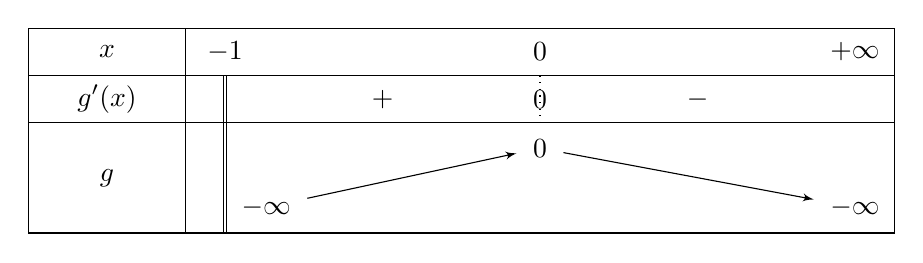
\begin{tikzpicture}
            \tkzTabInit[espcl=4]{$x$/0.6,$g'(x)$/0.6,$g$/1.4}{$-1$,0,$+\infty$}
            \tkzTabLine{d,+,z,-}
            \tkzTabVar{D-/$-\infty$, +/$0$, -/$-\infty$}
        \end{tikzpicture}
    \end{center}
    L'inégalité est donc vérifiée car ces fonctions prennent des valeurs négatives.
\end{tcolorbox}
\begin{tcolorbox}[enhanced, width=7in, center, size=fbox, fontupper=\large, drop shadow southwest]
    2. Soit $x\in]-1,+\infty[$. On a :
    \begin{equation*}
        \frac{x}{1+x}\leq\ln(1+x)\leq x
    \end{equation*}
    Et :
    \begin{equation*}
        \lim_{x\rightarrow0}\frac{1}{1+x}=1 \hspace{1cm} \text{et} \hspace{1cm} \lim_{x\rightarrow0}1=1
    \end{equation*}
    Donc, d'après le théorème des gendarmes :
   \begin{equation*}
        \lim_{x\rightarrow0}\frac{\ln(1+x)}{x}=1
   \end{equation*}
   3.
   On a :
   \begin{equation*}
        \lim_{x\rightarrow0}\frac{\ln(x+1)}{x}=\lim_{x\rightarrow0}\frac{\ln(x+1)-\ln(1)}{x}=\ln'(1)=\frac{1}{1}=1
   \end{equation*}
   \qed
\end{tcolorbox}
\addcontentsline{toc}{section}{\protect\numberline{}Exercice 4.5}

\section*{Exercice 4.6 [$\blacklozenge\blacklozenge\lozenge$]}
\begin{tcolorbox}[enhanced, width=7in, center, size=fbox, fontupper=\large, drop shadow southwest]
    Démontrer l'inégalité
    \begin{equation*}
        \forall{x\in\mathbb{R}_+}, \hspace{1cm} 0\leq x-\sin x\leq\frac{x^3}{6}.
    \end{equation*}
    Posons :
    \begin{equation*}
        f:x\mapsto x-\sin x \hspace{2cm} g:x\mapsto x-\sin x - \frac{x^3}{6}
    \end{equation*}
    Ces fonctions sont dérivables sur $\mathbb{R}_+$ :
    \begin{equation*}
        f':x\mapsto 1-\cos x \hspace {2cm} g':x\mapsto 1-\cos x - \frac{x^2}{2}
    \end{equation*}
    La première inégalité est triviale car $\cos x\leq1$, ainsi $x-\sin x\geq 0$.\\
    On a :
    \begin{equation*}
        g'':x\mapsto\sin x - x
    \end{equation*}
    Et donc :
    \begin{center}
        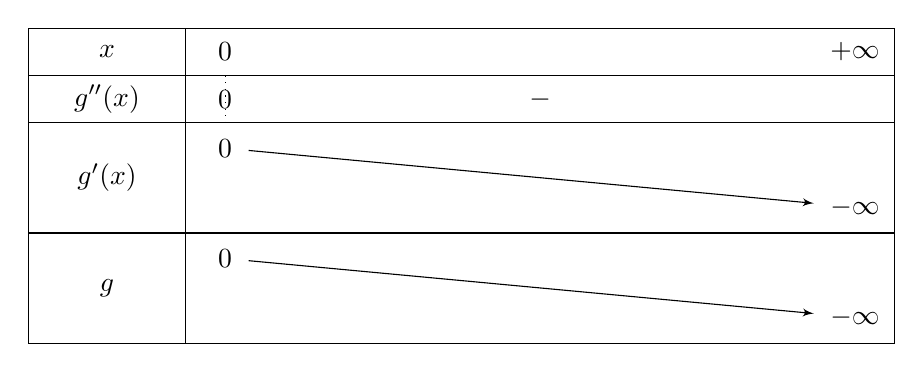
\begin{tikzpicture}
            \tkzTabInit[espcl=8]{$x$/0.6,$g''(x)$/0.6,$g'(x)$/1.4,$g$/1.4}{$0$,$+\infty$}
            \tkzTabLine{z,-}
            \tkzTabVar{+/$0$,-/$-\infty$}
            \tkzTabVar{+/$0$,-/$-\infty$}
        \end{tikzpicture}
    \end{center}
    Ainsi, $g$ prend des valeurs négatives sur $\mathbb{R}_+$, donc : $x-\sin x\leq\frac{x^3}{6}$.\\
    \qed
\end{tcolorbox}
\addcontentsline{toc}{section}{\protect\numberline{}Exercice 4.6}

\section*{Exercice 4.7 [$\blacklozenge\blacklozenge\lozenge$]}
\begin{tcolorbox}[enhanced, width=7in, center, size=fbox, fontupper=\large, drop shadow southwest]
    Faire une étude complète de la fonction 
    \begin{equation*}
        f:x\mapsto\ln\left(\left|\frac{1+x}{1-x}\right|\right)
    \end{equation*}
    $\circledcirc$ Soit $x\in]-1,1[$.\\
    On a :
    \begin{equation*}
        f:x\mapsto\ln\left(\frac{1+x}{1-x}\right) \hspace{2cm} f':x\mapsto\frac{2}{1-x^2}
    \end{equation*}
    $\circledcirc$ Soit $x\in]-\infty,-1[]1,+\infty[$.\\
    On a :
    \begin{equation*}
        f:x\mapsto\ln\left(-\frac{1+x}{1-x}\right) \hspace{2cm} f':x\mapsto\frac{2}{1-x^2}
    \end{equation*}
    Donc :
    \begin{equation*}
        \forall{x\in\mathbb{R}\setminus\{-1,1\}}, \hspace{1cm} f':x\mapsto\frac{2}{1-x^2}.
    \end{equation*}
    Ainsi,
    \begin{center}
        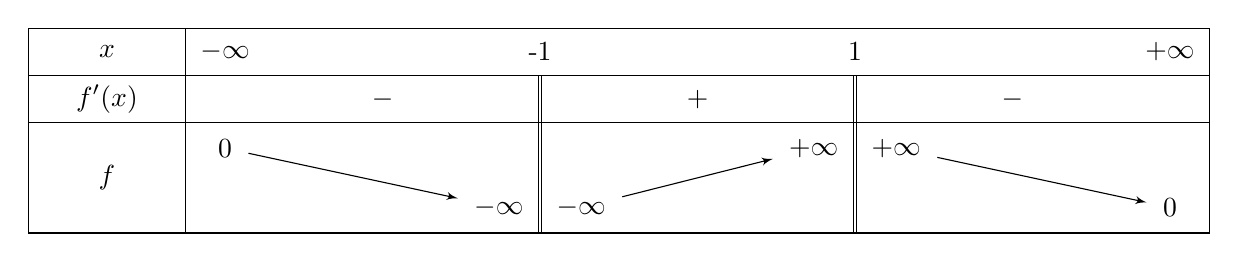
\begin{tikzpicture}
            \tkzTabInit[espcl=4]{$x$/0.6,$f'(x)$/0.6,$f$/1.4}{$-\infty$,-1,1,$+\infty$}
            \tkzTabLine{,-,d,+,d,-}
            \tkzTabVar{+/$0$,-D-/$-\infty$/$-\infty$,+D+/$+\infty$/$+\infty$,-/$0$}
        \end{tikzpicture}
    \end{center}
    \emph{Pour les limites :}
    \begin{equation*}
        f:x\mapsto\ln\left(\left|\frac{\frac{1}{x}+1}{\frac{1}{x}-1}\right|\right)
    \end{equation*}
\end{tcolorbox}
\addcontentsline{toc}{section}{\protect\numberline{}Exercice 4.7}

\section*{Exercice 4.8 [$\blacklozenge\blacklozenge\lozenge$]}
\begin{tcolorbox}[enhanced, width=7in, center, size=fbox, fontupper=\large, drop shadow southwest]
    Démontrer l'inégalité
    \begin{equation*}
        \forall{x\in]0,1[}\hspace{1cm}x^x(1-x)^{1-x}\geq\frac{1}{2}.
    \end{equation*}
    Soit $x\in]0,1[$.\\
    On a :
    \begin{equation*}
        x^x(1-x)^{1-x}=e^{x\ln x}e^{(1-x)\ln(1-x)}=e^{x\ln{x}+(1-x)\ln(1-x)}
    \end{equation*}
    Posons :
    \begin{equation*}
        f:x\mapsto e^{x\ln{x}+(1-x)\ln(1-x)} \hspace{1cm} f':x\mapsto \ln\left(\frac{x}{1-x}\right)e^{x\ln{x}+(1-x)\ln(1-x)}
    \end{equation*}
    \begin{center}
        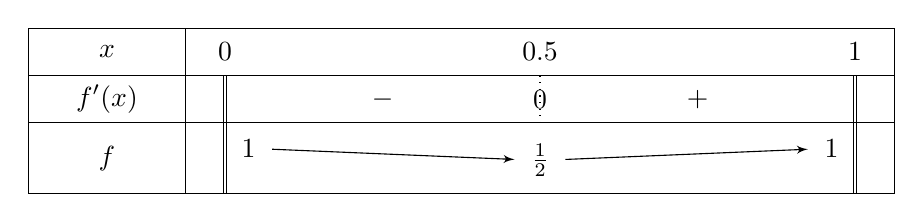
\begin{tikzpicture}
            \tkzTabInit[espcl=4]{$x$/0.6,$f'(x)$/0.6,$f$/0.9}{$0$,$0.5$,$1$}
            \tkzTabLine{d,-,z,+,d}
            \tkzTabVar{D+/$1$,-/$\frac{1}{2}$,+D/$1$}
        \end{tikzpicture}
    \end{center}
    \qed
\end{tcolorbox}
\addcontentsline{toc}{section}{\protect\numberline{}Exercice 4.8}

\section*{Exercice 4.9 [$\blacklozenge\blacklozenge\lozenge$]}
\begin{tcolorbox}[enhanced, width=7in, center, size=fbox, fontupper=\large, drop shadow southwest]
    1. Étudier les variations de $f:x\mapsto\frac{x}{1+x}$ sur $[0,+\infty[$.\\
    2. Prouver que
    \begin{equation*}
        \forall{x,y\in\mathbb{R}}, \hspace{1cm} \frac{|x+y|}{1+|x+y|}\leq\frac{|x|}{1+|x|}+\frac{|y|}{1+|y|}.
    \end{equation*}
    1. Soit $x\in\lbrack0,+\infty\lbrack$. On a :
    \begin{equation*}
        f':x\mapsto\frac{1}{(1+x)^2}
    \end{equation*}
    \begin{center}
        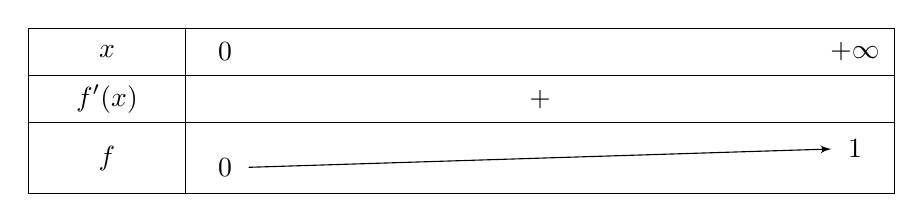
\begin{tikzpicture}
            \tkzTabInit[espcl=8]{$x$/0.6,$f'(x)$/0.6,$f$/0.9}{$0$,$+\infty$}
            \tkzTabLine{,+,}
            \tkzTabVar{-/$0$,+/$1$}
        \end{tikzpicture}
    \end{center}
    2. Soient $x,y\in\mathbb{R}$. Par inégalité triangulaire, on a :
    \begin{equation*}
        |x+y|\leq|x|+|y|
    \end{equation*}
    On applique $f$, fonction croissante sur $\mathbb{R}_+$, ce qui ne change pas les inégalités:
    \begin{align*}
        \frac{|x+y|}{1+|x+y|}&\leq\frac{|x|+|y|}{1+|x|+|y|}\\
        &\leq\frac{|x|}{1+|x|+|y|}+\frac{|y|}{1+|x|+|y|}\\
        &\leq\frac{|x|}{1+|x|}+\frac{|y|}{1+|y|}
    \end{align*}
    \qed
\end{tcolorbox}
\addcontentsline{toc}{section}{\protect\numberline{}Exercice 4.9}

\section*{Exercice 4.10 [$\blacklozenge\blacklozenge\lozenge$]}
\begin{tcolorbox}[enhanced, width=7in, center, size=fbox, fontupper=\large, drop shadow southwest]
    Soit la fonction $f:x\mapsto\ln\left(\sqrt{x^2+1}-x\right)$.\\
    1. Donner le domaine de définition de $f$.\\
    2. Montrer que $f$ est impaire.\\
    3. Étudier ses variations et donner le tableau correspondant.\\[0.25cm]
    1. Soit $g:\begin{cases}\mathbb{R}\rightarrow\mathbb{R}\\x\mapsto\sqrt{x^2+1}-x\end{cases}$ On a : $g':\begin{cases}\mathbb{R}\rightarrow\mathbb{R}\\x\mapsto\frac{x}{\sqrt{x^2+1}}-1\end{cases}$
    \begin{center}
        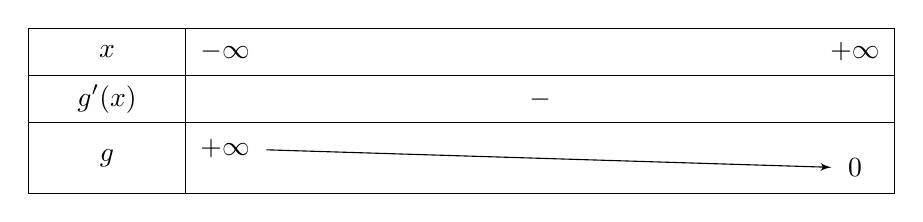
\begin{tikzpicture}
            \tkzTabInit[espcl=8]{$x$/0.6,$g'(x)$/0.6,$g$/0.9}{$-\infty$,$+\infty$}
            \tkzTabLine{,-,}
            \tkzTabVar{+/$+\infty$,-/$0$}
        \end{tikzpicture}
    \end{center}
    $f$ donc définie sur $\mathbb{R}$.
\end{tcolorbox}

\begin{tcolorbox}[enhanced, width=7in, center, size=fbox, fontupper=\large, drop shadow southwest]
    2. Soit $x\in\mathbb{R}$, on a :
    \begin{align*}
        -f(x)&=-\ln\left(\sqrt{x^2+1}-x\right)\\
        &=\ln\left(\frac{1}{\sqrt{x^2+1}-x}\right)\\
        &=\ln\left(\frac{\sqrt{x^2+1}+x}{x^2+1-x^2}\right)\\
        &=\ln\left(\sqrt{x^2+1}+x\right)\\
        &=f(-x)
    \end{align*}
    3. On a :
    \begin{equation*}
        f':\begin{cases}\mathbb{R}\rightarrow\mathbb{R}\\x\mapsto-\frac{1}{\sqrt{x^2+1}}\end{cases}
    \end{equation*}
    \begin{center}
        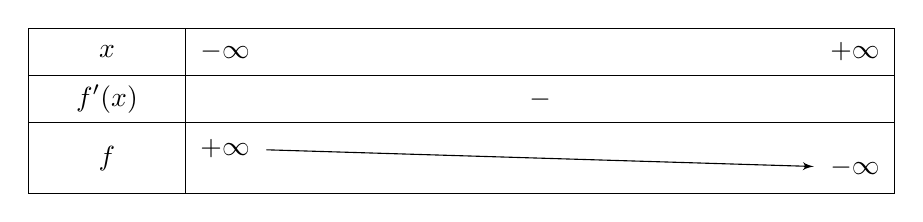
\begin{tikzpicture}
            \tkzTabInit[espcl=8]{$x$/0.6,$f'(x)$/0.6,$f$/0.9}{$-\infty$,$+\infty$}
            \tkzTabLine{,-,}
            \tkzTabVar{+/$+\infty$,-/$-\infty$}
        \end{tikzpicture}
    \end{center}
\end{tcolorbox}
\addcontentsline{toc}{section}{\protect\numberline{}Exercice 4.10}

\section*{Exercice 4.11 [$\blacklozenge\blacklozenge\lozenge$]}
\begin{tcolorbox}[enhanced, width=7in, center, size=fbox, fontupper=\large, drop shadow southwest]
    Notons $a$ le nombre
    \begin{equation*}
        \sqrt[3]{20+14\sqrt{2}}+\sqrt[3]{20-14\sqrt{2}}.
    \end{equation*}
    1. Montrer que $a^3=6a+40$.\\
    2. En déduire la valeur de $a$.\\[0.25cm]
    1.
    \begin{align*}
        a^3&=40+3\sqrt[3]{(20+14\sqrt{2})^2(20-14\sqrt{2})}+3\sqrt[3]{(20+14\sqrt{2})(20-14\sqrt{2})^2}\\
        &=40+3\sqrt[3]{(20+14\sqrt{2})(400-392)}+3\sqrt[3]{(20-14\sqrt{2})(400-392)}\\
        &=40+6\sqrt[3]{20+14\sqrt{2}}+6\sqrt[3]{20-14\sqrt{2}}\\
        &=6a+40
    \end{align*}
    2. On a :
    \begin{align*}
        &a^3-6a-40=0\\
        \iff&(a-4)(a^2+4a+10)=0\\
        \iff&a=4
    \end{align*}
\end{tcolorbox}
\addcontentsline{toc}{section}{\protect\numberline{}Exercice 4.11}

\section*{Exercice 4.12 [$\blacklozenge\lozenge\lozenge$]}
\begin{tcolorbox}[enhanced, width=7in, center, size=fbox, fontupper=\large, drop shadow southwest]
    Considérons la fonction
    \begin{equation*}
        f:\begin{cases}\rbrack1,+\infty\lbrack\rightarrow\mathbb{R}\\x\mapsto\exp(-\frac{1}{\ln(x)})\end{cases}.
    \end{equation*}
    1. Démontrer que $f$ réalise une bijection de $\rbrack1,+\infty\lbrack$ dans un intervalle que l'on précisera.\\
    2. Expliciter la réciproque de $f$. Peut-on écrire en conclusion que $f^{-1}=f$ ?\\[0.25cm]
    Soit $x\in\rbrack1,+\infty\lbrack$ et $y\in\mathbb{R}^*_+$. On a :
    \begin{align*}
        &y=f(x)\\
        \iff& y=\exp(-\frac{1}{\ln(x)})\\
        \iff& \ln(y)=-\frac{1}{\ln(x)}\\
        \iff& -\frac{1}{\ln(y)}=\ln(x)\\
        \iff& x=\exp(-\frac{1}{\ln(y)})
    \end{align*}
    L'équation a une unique solution, $f$ réalise donc une bijection de $\rbrack1,+\infty\lbrack$ vers $\mathbb{R}^*_+$.\\
    2. On a :
    \begin{equation*}
        f^{-1}:\begin{cases}\mathbb{R}^*_+\rightarrow\rbrack1,+\infty\lbrack\\x\mapsto\exp(-\frac{1}{\ln(x)})\end{cases}
    \end{equation*}
    $f\neq f^{-1}$ car leurs domaines de définition sont différents.
\end{tcolorbox}
\addcontentsline{toc}{section}{Bijections.}
\addcontentsline{toc}{section}{\protect\numberline{}Exercice 4.12}

\section*{Exercice 4.13 [$\blacklozenge\blacklozenge\blacklozenge$]}
\begin{tcolorbox}[enhanced, width=7in, center, size=fbox, fontupper=\large, drop shadow southwest]
    1. Montrer que $\tah$ est une bijection de $\mathbb{R}$ dans $\rbrack-1,1\lbrack$ et déterminer une expression explicite de sa réciproque, qu'on notera $\argth$.\\
    2. De deux façons différentes, montrer que $\argth$ est dérivable sur son intervalle de définition et calculer sa dérivée.\\
    3. Montrer que pour tout $x\in\mathbb{R}$, $\argth\left(\frac{1+3\tah x}{3+\tah x}\right)=x+\ln\sqrt{2}$.\\[0.25cm]
    1. Soit $x\in\mathbb{R}$ et $y\in\rbrack-1,1\lbrack$. On a :
    \begin{align*}
        &y=\tah x\\
        \iff& y=\frac{e^x-e^{-x}}{e^x+e^{-x}}\\
        \iff& y=\frac{e^{2x}-1}{e^{2x}+1}\\
        \iff& e^{2x}(1-y)=y+1\\
        \iff &e^{2x}=\frac{y+1}{1-y}\\
        \iff &x=\frac{1}{2}\ln\left(\frac{y+1}{1-y}\right)
    \end{align*}
    L'équation a une unique solution, $\tah$ réalise donc une bijection de $\mathbb{R}$ dans $\rbrack-1,1\lbrack$.\\
    Sa réciproque est $\argth:\begin{cases}\rbrack-1,1\lbrack\rightarrow\mathbb{R}\\x\mapsto\frac{1}{2}\ln\left(\frac{x+1}{1-x}\right)\end{cases}$\\[0.25cm]
    2. On peut montrer que $\argth$ est dérivable sur $]-1,1[$ par le théorème de dérivée des réciproques ou en dérivant $x\mapsto\frac{1}{2}\ln\left(\frac{x+1}{1-x}\right)$ comme composée de fonctions dérivables.\\
    On retrouve dans les deux cas:
    \begin{equation*}
        \argth':\begin{cases}]-1,1[\rightarrow\mathbb{R}\\x\mapsto\frac{1}{1-x^2}\end{cases}
    \end{equation*}
    3. Soit $x\in\mathbb{R}$.
    \begin{align*}
        \argth\left(\frac{1+3\tah x}{3+\tah x}\right)&=\frac{1}{2}\ln\left(\frac{\frac{1+3\tah x}{3+\tah x}+1}{1-\frac{1+3\tah x}{3+\tah x}}\right)\\
        &=\frac{1}{2}\ln\left(\frac{\frac{4+4\tah x}{3+\tah x}}{\frac{2-2\tah x}{3 + \tah x}}\right)\\
        &=\frac{1}{2}\ln\left(\frac{2+2\tah x}{1-\tah x}\right)\\
        &=\frac{1}{2}\ln\left(\frac{\ch(x)+\sh(x)}{\ch(x)-\sh(x)}\right)+\frac{1}{2}\ln(2)\\
        &=\frac{1}{2}\ln\left(e^{2x}\right)+\ln(\sqrt{2})\\
        &=x+\ln\sqrt{2}
    \end{align*}
    \qed
\end{tcolorbox}

\addcontentsline{toc}{section}{\protect\numberline{}Exercice 4.13}
\end{document}
